\exercisesheader{}

% 1 - distribution_p_hat_1

\eoce{\qt{Distribution of $\pmb{\hat{p}}$\label{distribution_p_hat_1}} Suppose the true population proportion were $p = 0.95$. The figure below shows what the distribution of a sample proportion looks like when the sample size is $n = 20$, $n = 100$, and $n = 500$. (a) What does each point (observation) in each of the samples represent? (b) Describe the distribution of the sample proportion, $\hat{p}$. How does the distribution of the sample proportion change as $n$ becomes larger?
\begin{center}
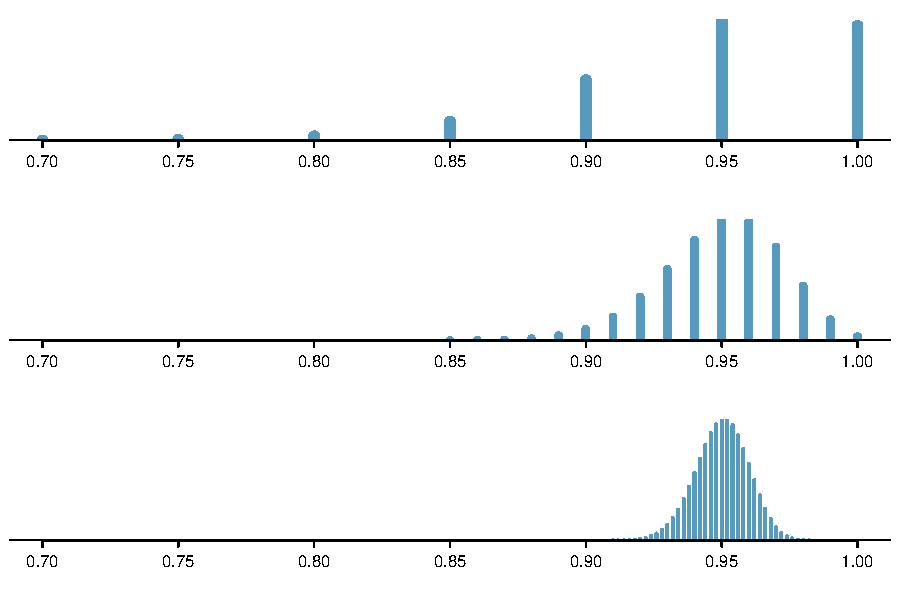
\includegraphics[width=0.85\textwidth]{ch_distributions/figures/eoce/distribution_p_hat_1/eoce-p-hat-simulations-p95}
\end{center}
}{}

% 2 - distribution_p_hat_2

\eoce{\qt{Distribution of $\pmb{\hat{p}}$\label{distribution_p_hat_2}} Suppose the true population proportion were $p = 0.5$. The figure below shows what the distribution of a sample proportion looks like when the sample size is $n = 20$, $n = 100$, and $n = 500$. What does each point (observation) in each of the samples represent? Describe how the distribution of the sample proportion, $\hat{p}$, changes as $n$ becomes larger.
\begin{center}
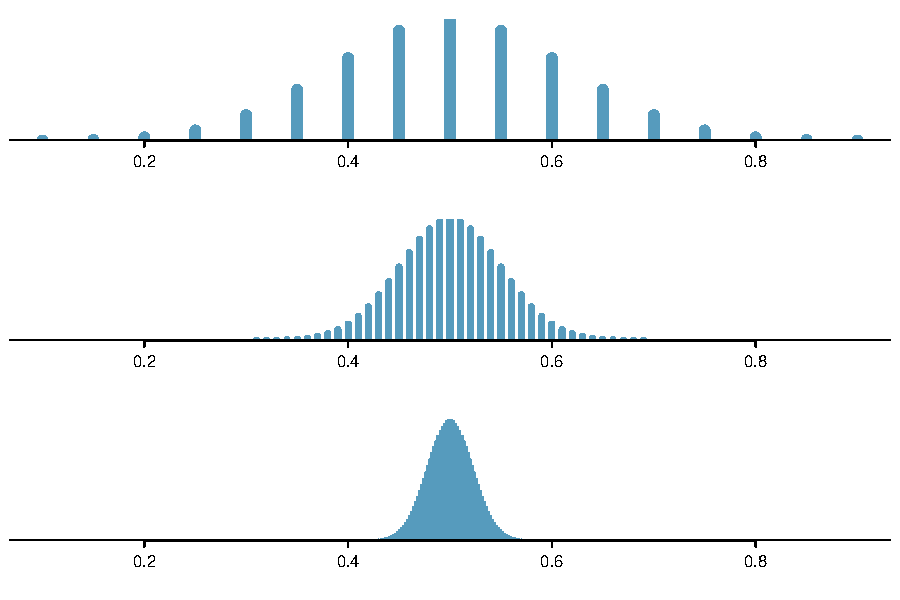
\includegraphics[width=0.85\textwidth]{ch_distributions/figures/eoce/distribution_p_hat_2/eoce-p-hat-simulations-p5}
\end{center}
}{}

% 3 - veg_coll_students_CLT

\eoce{\qt{Vegetarian college students\label{veg_coll_students_CLT}} Suppose that 8\% 
of college students are vegetarians. Determine if the following statements are 
true or false, and explain your reasoning.
\begin{parts}
\item The distribution of the sample proportions of vegetarians in random 
samples of size 60 is approximately normal since $n \ge 30$. 
\item The distribution of the sample proportions of vegetarian college 
students in random samples of size 50 is right skewed.
\item A random sample of 125 college students where 12\% are vegetarians 
would be considered unusual. 
\item A random sample of 250 college students where 12\% are vegetarians 
would be considered unusual.
\item The standard error would be reduced by one-half if we increased the 
sample size from 125 to~250.
\end{parts}
 
}{}

% 4 - young_americans_CLT_1

\eoce{\qt{Young Americans, Part I\label{young_americans_CLT_1}} About 77\% of 
young adults think they can achieve the American dream. Determine if the 
following statements are true or false, and explain your reasoning.
\footfullcite{news:youngAmericans1}
\begin{parts}
\item The distribution of sample proportions of young Americans who think 
they can achieve the American dream in random samples of size 20 is left skewed.
\item The distribution of sample proportions of young Americans who think 
they can achieve the American dream in random samples of size 40 is 
approximately normal since $n \ge 30$. 
\item A random sample of 60 young Americans where 85\% think they can achieve 
the American dream would be considered unusual.
\item A random sample of 120 young Americans where 85\% think they can 
achieve the American dream would be considered unusual.
\end{parts}
}{}

% 5 - distribution_p_hat_3

\eoce{\qt{Distribution of $\pmb{\hat{p}}$\label{distribution_p_hat_3}} \videosolution{ahss_eoce_sol-distribution_of_phat} Suppose the true population proportion were $p = 0.5$ and a researcher takes a simple random sample of size $n=50$.  
\begin{parts}
\item Find and interpret the standard deviation of the sample proportion $\hat{p}$.  
\item Calculate the probability that the sample proportion will be larger than 0.55 for a random sample of size 50.
\end{parts}
}{}

% 6 - distribution_p_hat_4

\eoce{\qt{Distribution of $\pmb{\hat{p}}$\label{distribution_p_hat_4}} Suppose the true population proportion were $p = 0.6$ and a researcher takes a simple random sample of size $n=50$.  
\begin{parts}
\item Find and interpret the standard deviation of the sample proportion $\hat{p}$. 
\item Calculate the probability that the sample proportion will be larger than 0.65 for a random sample of size 50.
\end{parts}
}{}

% 7 - nearsighted_children

\eoce{\qt{Nearsighted children\label{nearsighted_children}} \videosolution{ahss_eoce_sol-nearsighted_children} It is believed that nearsightedness affects about 8\% of all children. We are interested in finding the probability that fewer than 12 out of 200 randomly sampled children will be nearsighted.
\begin{parts}
\item Estimate this probability using the normal approximation to the binomial distribution.
\item Estimate this probability using the distribution of the sample proportion.
\item How do your answers from parts (a) and (b) compare?
\end{parts}
}{}

% 8 - social_network_use

\eoce{\qt{Social network use\label{social_network_use}} The Pew Research Center estimates that as of January 2014, 89\% of 18-29 year olds in the United States use social networking sites.\footfullcite{data:pewsocialnetwork:2014} Calculate the probability that at least 95\% of 500 randomly sampled 18-29 year olds use social networking sites.
}{}

% 9 - CLT_prop_pt1

\eoce{\qt{CLT for proportions, Part 1\label{CLT_prop_pt1}}
Define the term ``sampling distribution" of the sample proportion,
and describe how the shape, center, and spread of the sampling
distribution change as the sample size increases when $p = 0.1$.
}{}

% 10 - CLT_prop_pt2

\eoce{\qt{CLT for proportions, Part 2\label{CLT_prop_pt2}}
Define the term ``sampling distribution" of the sample proportion,
and describe how the shape, center, and spread of the sampling
distribution change as the sample size increases when $p = 0.8$.
}{}
